\chapter{Getting started with \spriteb{} 1.0}
Spritebuilder is a tool that derived from Cocosbuilder which originally was
written by Victor Lidholt at Zynga. The goal of Spritebuilder is to provide a
WYSIWYG editor for \cocos{} games. 

In the creation of many scenes you can save a lot of time if you don't
have to layout your menus in code, and instead can place them visually.

If you decide to you use \spriteb{}, you will start your game by creating a new
\spriteb{} project instead of starting of with a Xcode project. Whenever you
start a new \spriteb{} project, it will create and maintain a Xcode project for
you.

Similar to Xcode's Interface Builder you will create interface files using
\spriteb{} and you will be able to connect the interface files with classes you
have created in Xcode.

Interface files in \spriteb{} are called \textit{CCB} files. Each 
CCB file maintains a own scene graph. This means a CCB file can be interpreted
as a CCScene or a CCNode.

If you work on a project using \spriteb{} you workflow will look like this:
\begin{itemize}
  \item Create a project in \spriteb{}
  \item Add images and other resources to your \spriteb{} project.
  \item Create multiple CCB files for the different scenes in your project.
  \item \textbf{Publish} your project in \spriteb{}. This will create or update
  the Xcode project related to your \spriteb{}. 
  \item Add code to your classes in Xcode.
\end{itemize}

Here's a diagram that shows how \spriteb{} and Xcode work together in your
\spriteb{} projects:

\begin{figure}[H]
		\centering
		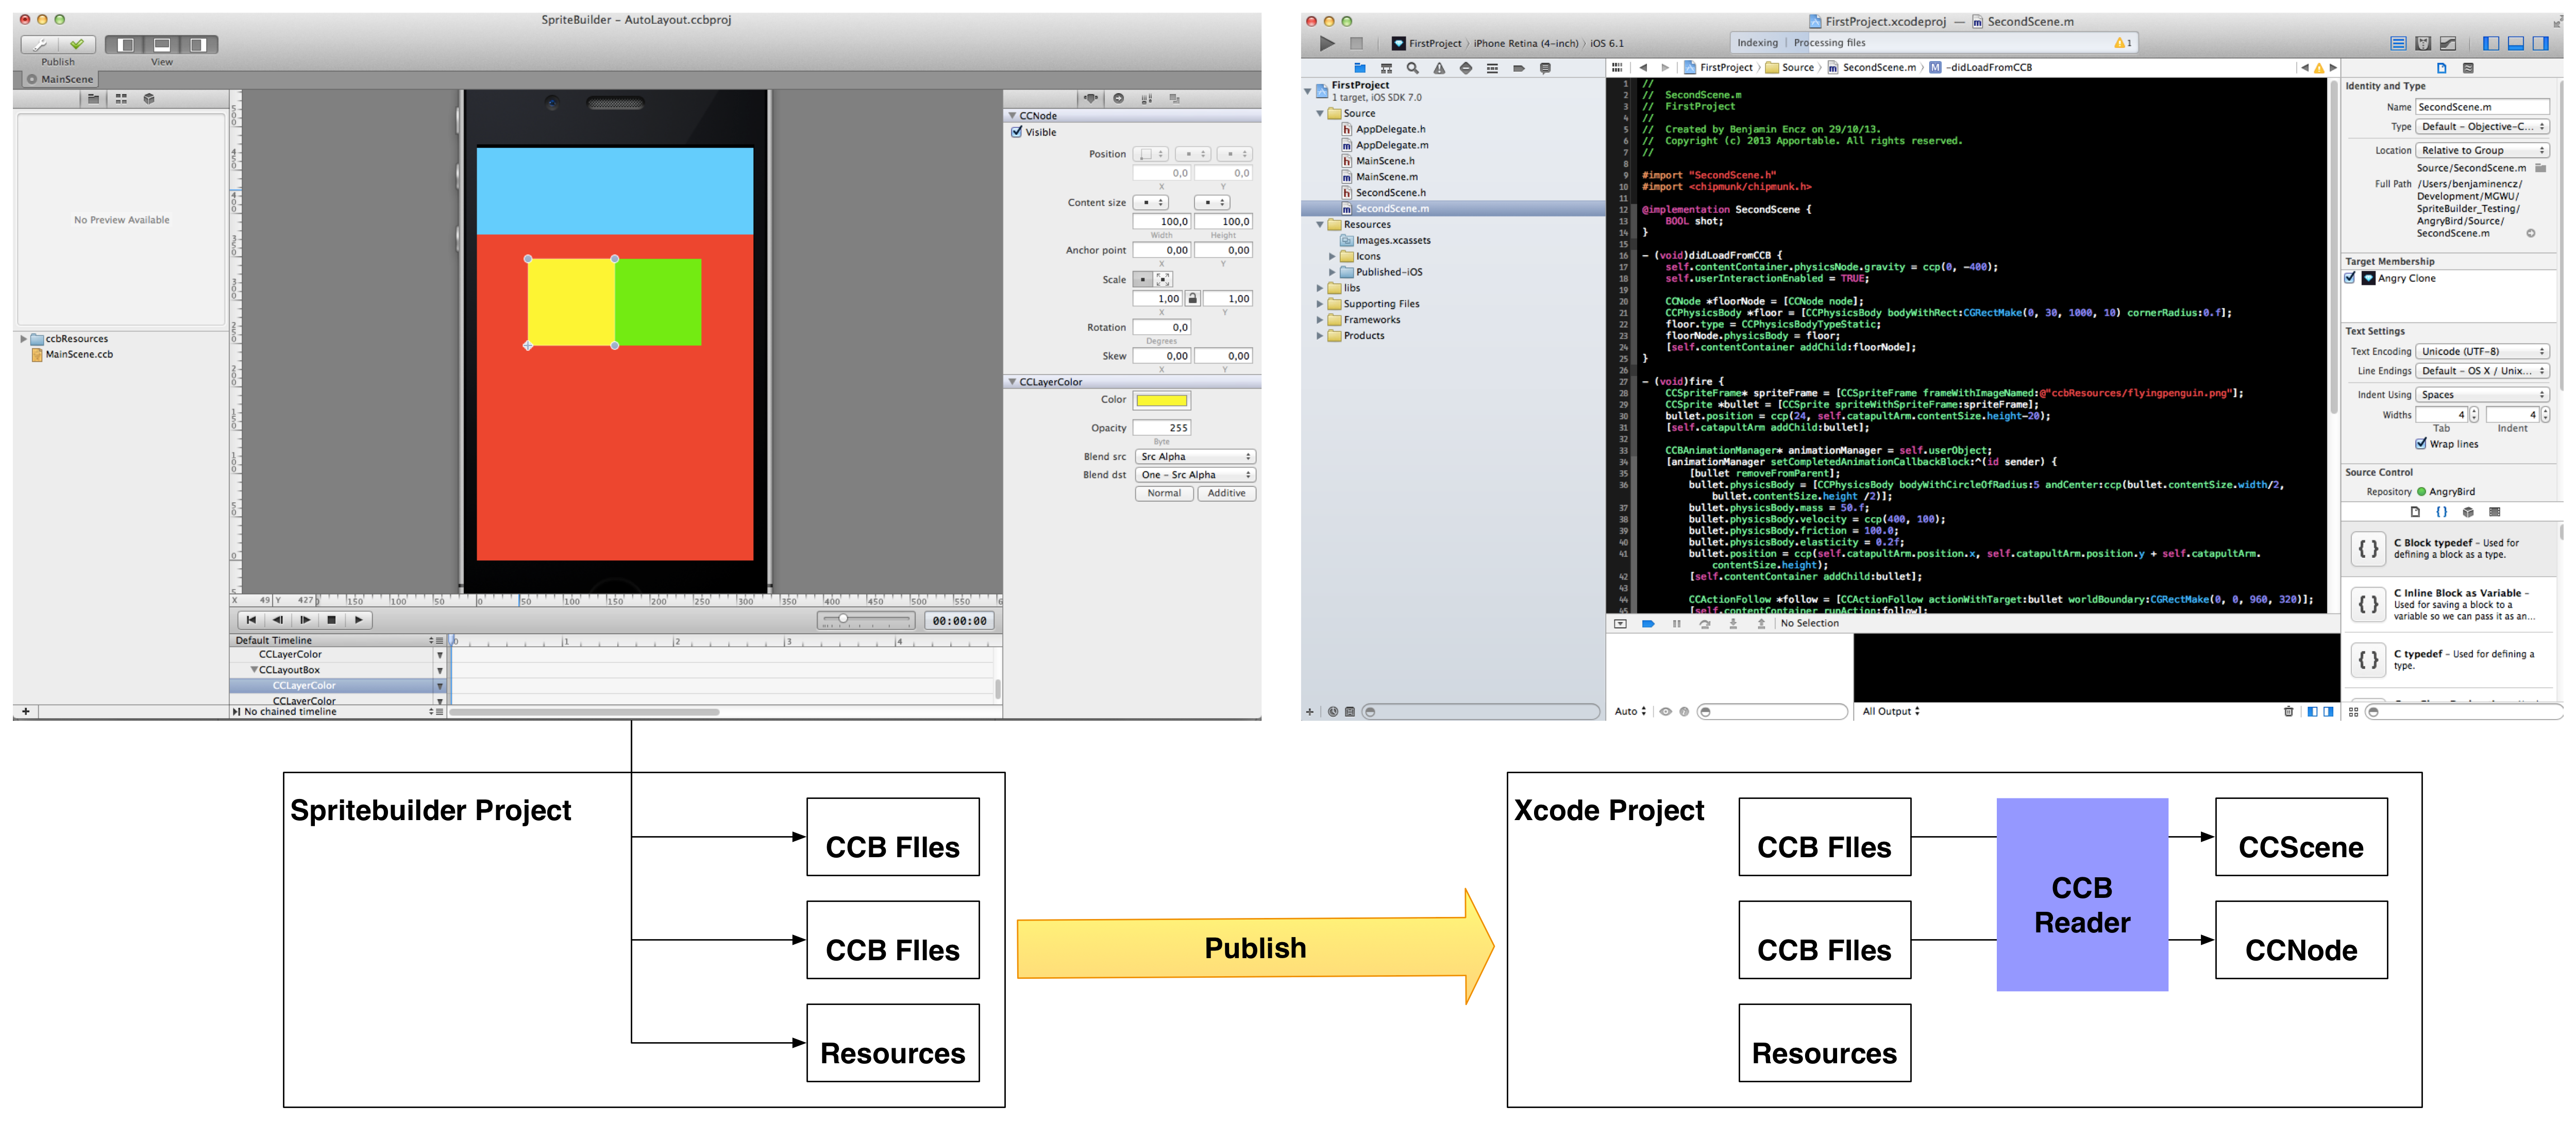
\includegraphics[width=400pt]{images/spritebuilder_publishing.png}     
		\caption{Spritebuilder creates and organizes a Xcode project for you. Adding
		all the resources and scenes you have created.}
		%\label{labelstruct} 
\end{figure}

For those that are interested in a behind the scenes tour, I will give a short
explanation of how \spriteb{} works. In \spriteb{} you create CCB Files, these
store a scene graph; the hierarchy and positions of your nodes. When publishing
in \spriteb the CCB Files and all other resources stored in your \spriteb{}
project are copied to your Xcode project.
When running the project in Xcode a class called CCBReader wil parse your CCB
files and create the according CCNode subclasses to reconstruct the scene graph
you have designed in \spriteb{}.

When you use \spriteb{}, you still implement the navigation in code. The highest
level you will be using CCB files at, are one scene. 
Ok, now let's start by creating our first project using \spriteb{}!

\section{The first Spritebuilder project}
Open \spriteb{} and select \textit{File->New->Project}. Select a folder for your
new project. 

\begin{figure}
		\centering
		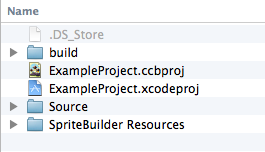
\includegraphics[width=100pt]{images/spritebuilder_project_folderstructure.png}     
		\caption{Typical folder structure after creating a Spritebuilder project. You
		have a \spriteb{} project (.ccbproj)  and a Xcode project (.xcodeproj)}
		%\label{labelstruct} 
\end{figure}

\section{The Spritebuilder User Interface}

\section{Layouting in Spritebuilder}

\section{Custom classes in Spritebuilder}
- How custom classes for scenes?

\section{Inheritance using Spritebuilder}